% Build from this folder: pdflatex update_report.tex (twice), then copy the PDF to others/update_report.pdf.
\documentclass[conference]{IEEEtran}
\usepackage{amsmath,amssymb}
\usepackage{graphicx}
\usepackage{booktabs}
\usepackage{url}
\usepackage{cite}
\usepackage{tikz}
\usetikzlibrary{arrows.meta,positioning}
\graphicspath{{./}{../../data/results/}}

% Course header above the top margin of page 1 (the manual forbids a title page).
\makeatletter
\def\ps@IEEEtitlepagestyle{%
  \def\@oddhead{\parbox[b]{\textwidth}{\centering\fontsize{7.8}{9.4}\selectfont
    CSE 440 (Section 1) \quad$\vert$\quad Group 2\\
    Md Shihabul Alam Shihab (2233115642) \;$\cdot$\; Rayed Riasat Rabbi (2311649042) \;$\cdot$\;
    Rifat Imtiaze Ruddro (2311474642) \;$\cdot$\; Sayma Akhter Snigdha (1620838042)}}%
  \def\@evenhead{}\def\@oddfoot{}\def\@evenfoot{}}
\makeatother

\newcommand{\algo}[1]{\texttt{#1}}

\begin{document}
\title{LogicPuzzleX: One Constraint Engine for Sudoku and Kakuro}
\author{\IEEEauthorblockN{Md Shihabul Alam Shihab, Rayed Riasat Rabbi, Rifat Imtiaze Ruddro, Sayma Akhter Snigdha}
\IEEEauthorblockA{Department of ECE, North South University}}
\maketitle

\section{Introduction}
Logic puzzles such as Sudoku and Kakuro are constraint satisfaction problems (CSPs): assign a value to every variable so that every constraint holds~\cite{aima}. Generalized Sudoku is NP-complete~\cite{yato}, yet good CSP techniques solve typical $9\times9$ puzzles in milliseconds. LogicPuzzleX models each puzzle as a factor graph, solves it with a ladder of increasingly capable algorithms and shows the search live in the browser. We measure what each technique contributes and compare CSP search with propositional logic on the same task. Four questions drive the work:

\noindent\textbf{RQ1:} How much does each technique cut search effort and runtime?
\textbf{RQ2:} Does solver effort predict rated difficulty, and how many puzzles need no search?
\textbf{RQ3:} How do binary, global and CNF formulations compare?
\textbf{RQ4:} How does one engine scale from $4\times4$ to $16\times16$ Sudoku, and to Kakuro?

\section{Approach}
A puzzle is a factor graph: variables $X_i$ with domains, and factors $f_j(x)\in\{0,1\}$. A complete assignment $x$ solves it when
\begin{equation}
  \mathrm{weight}(x)=\prod_{j=1}^{m} f_j(x)=1 .
\end{equation}
A $9\times9$ Sudoku has 81 variables and 810 binary $\neq$ factors, or 27 global AllDifferent factors. Givens are fixed by conditioning, and a cell's 20 peers form its Markov blanket. Search extends a partial assignment $x$ with $X_i=v$ only if every dependent factor in $D(x,X_i)$ stays satisfied~\cite{notes}:
\begin{equation}
  \delta(x,X_i,v)=\prod_{f\in D(x,X_i)} f\bigl(x\cup\{X_i:v\}\bigr)=1 .
\end{equation}
One recursive search serves the whole ladder in Table~\ref{tab:ladder}: each rung changes only the variable order, the value order or the inference step. The logic track encodes the same puzzle in CNF~\cite{lynce} with 729 symbols and 11,745 clauses, and solves it with DPLL~\cite{dpll}. A solution $s$ is unique exactly when $\mathrm{KB}\cup\{\neg s\}$ is unsatisfiable, that is, when $\mathrm{KB}\models s$. Fig.~\ref{fig:arch} shows how the parts connect: every solver emits the same event stream, and that stream drives every animation in the app.

\begin{table}[t]
\caption{The algorithm ladder}
\label{tab:ladder}
\centering\footnotesize
\begin{tabular}{@{}llll@{}}
\toprule
ID & Variable order & Value order & Inference \\
\midrule
\algo{bt}   & static          & ascending  & none \\
\algo{fc}   & static          & ascending  & forward checking~\cite{haralick} \\
\algo{mrv}  & MRV, degree     & ascending  & forward checking \\
\algo{lcv}  & MRV, degree     & LCV        & forward checking \\
\algo{mac}  & MRV, degree     & LCV        & AC-3~\cite{mackworth} \\
\algo{mac+} & MRV, degree     & LCV        & AC-3, hidden singles~\cite{simonis} \\
\algo{dpll} & shortest clause & true first & unit propagation~\cite{dpll} \\
\bottomrule
\end{tabular}
\end{table}

\begin{figure}[t]
\centering
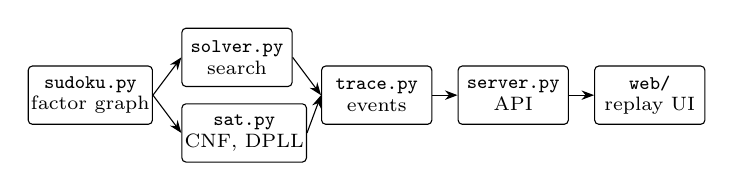
\begin{tikzpicture}[
    box/.style={draw, rounded corners=1.5pt, minimum width=14mm, minimum height=7.4mm, inner sep=1pt,
                align=center, font=\fontsize{6.8}{7.8}\selectfont},
    arrow/.style={-{Stealth[length=1.6mm]}, thin},
    node distance=3.2mm]
  \node[box] (model) {\texttt{sudoku.py}\\factor graph};
  \node[box, right=3.6mm of model, yshift=4.8mm] (solver) {\texttt{solver.py}\\search};
  \node[box, right=3.6mm of model, yshift=-4.8mm] (sat) {\texttt{sat.py}\\CNF, DPLL};
  \node[box, right=3.6mm of solver, yshift=-4.8mm] (trace) {\texttt{trace.py}\\events};
  \node[box, right=of trace] (server) {\texttt{server.py}\\API};
  \node[box, right=of server] (web) {\texttt{web/}\\replay UI};
  \draw[arrow] (model.east) -- (solver.west);
  \draw[arrow] (model.east) -- (sat.west);
  \draw[arrow] (solver.east) -- (trace.west);
  \draw[arrow] (sat.east) -- (trace.west);
  \draw[arrow] (trace) -- (server);
  \draw[arrow] (server) -- (web);
\end{tikzpicture}
\caption{Architecture. Both solver families feed one event stream.}
\label{fig:arch}
\end{figure}

\section{Progress}
All of Sudoku already works end to end, ahead of the minimal version planned for this update. All seven algorithms run on $4\times4$, $6\times6$, $9\times9$ and $16\times16$ grids, and 166 automated tests pass. The generator produces puzzles of a requested grade with exactly one solution, and Explain mode turns solver events into plain-English deductions. In the browser app (Fig.~\ref{fig:app}) a user can play with live solvability checks and hints, replay the search, race up to four algorithms and browse the benchmarks. Kakuro is the main work left: its sum factors, propagation and board, which RQ4 needs. The demo video, a README GIF and the final report also remain.

\begin{figure*}[t]
\centering
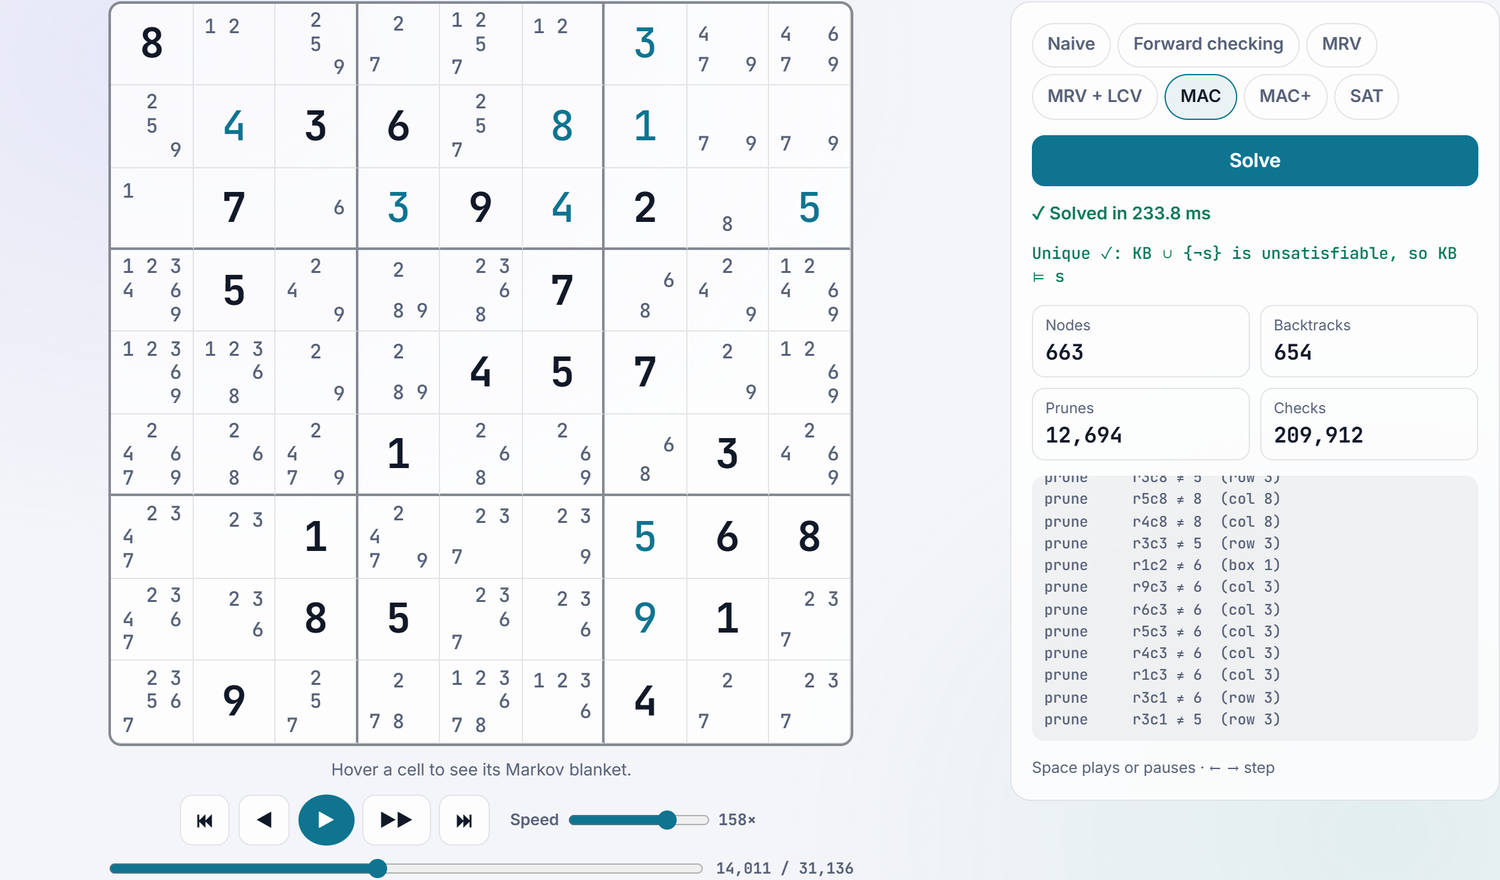
\includegraphics[width=0.76\textwidth]{app_screenshot.png}
\caption{``Watch it think'' part-way through a replay of \algo{mac} on Inkala's 2012 puzzle, with the SAT uniqueness proof above the statistics.}
\label{fig:app}
\end{figure*}

\section{Preliminary Results}
We ran each algorithm on 1000 puzzles, 250 per difficulty bucket, sampled from a rated dataset of 3 million~\cite{radcliffe}, with a 10\,s limit per run and the median of 3 timed runs on a 4-vCPU Kaggle session (Fig.~\ref{fig:nodes}). MRV gives the largest single gain, 23$\times$ fewer nodes than forward checking (paired median), while LCV adds nothing here (Table~\ref{tab:results}). MAC roughly halves the nodes again yet runs slower than MRV (median 44\,ms against 27\,ms). Hidden singles give the fastest solver: \algo{mac+} takes a median 24\,ms and needs no backtracking on any puzzle in the easy bucket.

Naive backtracking times out on 33\% of puzzles, and at similar rates in every bucket (30--36\%), so its failures barely follow difficulty. Rank correlation between rating and nodes peaks at $\rho=0.475$ for \algo{mac+}; the rating comes from an automated solver rather than from people, so this is not direct evidence about human difficulty. Global factors halve MAC's time without changing its search, and 243 redundant clauses cut DPLL's nodes sixfold. On 8 generated $16\times16$ puzzles only \algo{mac+} finished (median 208\,ms); the other six hit the limit on all 8.

\begin{figure}[t]
\centering
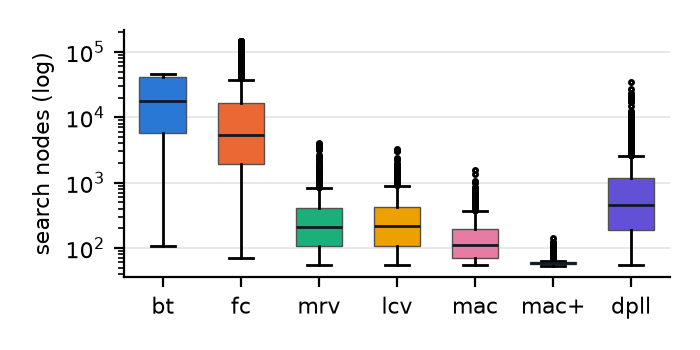
\includegraphics[width=\columnwidth]{e1_overview.png}
\caption{Search nodes per algorithm on 1000 rated puzzles. A run that hits the 10\,s limit counts the nodes it reached, so \algo{bt} and \algo{fc} are lower bounds.}
\label{fig:nodes}
\end{figure}

\begin{table}[t]
\caption{Median effort on 1000 rated puzzles}
\label{tab:results}
\centering\footnotesize
\begin{tabular}{@{}lrrr@{}}
\toprule
ID & Nodes & Time (ms) & Timed out \\
\midrule
\algo{bt}   & 17,890 & 4,185 & 32.9\% \\
\algo{fc}   & 5,446  & 406   & 2.3\% \\
\algo{mrv}  & 210    & 27    & 0\% \\
\algo{lcv}  & 219    & 30    & 0\% \\
\algo{mac}  & 113    & 44    & 0\% \\
\algo{mac+} & 58     & 24    & 0\% \\
\algo{dpll} & 448    & 103   & 0\% \\
\bottomrule
\end{tabular}
\end{table}

\begin{table}[t]
\caption{Course concept map}
\label{tab:concepts}
\centering\footnotesize
\begin{tabular}{@{}llc@{}}
\toprule
Feature & Course concept & Vol. \\
\midrule
Puzzle to variables and factors & Factor graphs, CSP & 3 \\
Givens fixed before search & Conditioning & 3 \\
A cell and its 20 peers & Markov blanket & 3 \\
Search over partial assignments & Backtracking, DFS & 1 \\
Forward checking, AC-3 & Constraint propagation & 3 \\
Sudoku to CNF, DPLL & Propositional logic & 4 \\
Uniqueness proof & Entailment & 4 \\
Explain mode & Inference rules & 4 \\
\bottomrule
\end{tabular}
\end{table}

\section{Plan to Final}
\noindent\textbf{3--16 Nov:} Kakuro on the same engine, with sum factors and a board in the app.
\textbf{17--30 Nov:} Kakuro in the scaling experiment, README GIF, feature freeze.
\textbf{December:} 8-page report, final slides, one-minute video and rehearsals.

\noindent\textbf{AI use:} Claude Code~\cite{claude} assisted with planning, code, experiments and drafting this report.

\begin{thebibliography}{10}
\footnotesize
\bibitem{aima} S. Russell and P. Norvig, \emph{Artificial Intelligence: A Modern Approach}, 4th ed. Pearson, 2020.
\bibitem{yato} T. Yato and T. Seta, ``Complexity and completeness of finding another solution and its application to puzzles,'' \emph{IEICE Trans. Fundamentals}, vol. E86-A, no. 5, 2003.
\bibitem{notes} CSE 440 course notes, Vols. 1--4, North South University, 2026.
\bibitem{lynce} I. Lynce and J. Ouaknine, ``Sudoku as a SAT problem,'' in \emph{Proc. ISAIM}, 2006.
\bibitem{dpll} M. Davis, G. Logemann, and D. Loveland, ``A machine program for theorem-proving,'' \emph{Commun. ACM}, vol. 5, no. 7, pp. 394--397, 1962.
\bibitem{haralick} R. M. Haralick and G. L. Elliott, ``Increasing tree search efficiency for constraint satisfaction problems,'' \emph{Artif. Intell.}, vol. 14, no. 3, pp. 263--313, 1980.
\bibitem{mackworth} A. K. Mackworth, ``Consistency in networks of relations,'' \emph{Artif. Intell.}, vol. 8, no. 1, pp. 99--118, 1977.
\bibitem{simonis} H. Simonis, ``Sudoku as a constraint problem,'' in \emph{CP Workshop on Modeling and Reformulating CSPs}, 2005.
\bibitem{radcliffe} D. Radcliffe, ``3 million Sudoku puzzles with ratings,'' Kaggle dataset, CC0-1.0, accessed Oct. 2026. [Online]. Available: \url{https://www.kaggle.com/datasets/radcliffe/3-million-sudoku-puzzles-with-ratings}
\bibitem{claude} Anthropic, Claude Code (Claude Opus 5.5), AI assistant used for planning, code, experiments and drafting this report, Oct. 2026.
\end{thebibliography}
\end{document}
